\documentclass{beamer}
%\documentclass[handout]{beamer}
\usepackage[hungarian]{babel}
\uselanguage{hungarian}
\languagepath{hungarian}
\deftranslation[to=hungarian]{Theorem}{T\'etel}
\deftranslation[to=hungarian]{Example}{P\'elda}
\deftranslation[to=hungarian]{Definition}{Defin\'ici\'o}
%\usepackage[magyar]{babel}
\usepackage[utf8]{inputenc}
\usepackage[T1]{fontenc}
\usepackage{beamerthemesplit}
\usepackage{pgf,pgffor,pgfplots}
\pgfplotsset{compat=1.15}
\usepackage{subfig}
\usepackage{xcolor}
\usepackage{nccfoots}
\newcommand{\framenote}[1]{%
	\Footnotetext{}{\emph{#1}}% Print footnote text
}
\usepackage{lstlinebgrd}
\AtBeginEnvironment{figure}{\setcounter{subfigure}{0}}
\makeatletter
%%%%%%%%%%%%%%%%%%%%%%%%%%%%%%%%%%%%%%%%%%%%%%%%%%%%%%%%%%%%%%%%%%%%%%%%%%%%%%
%
% \btIfInRange{number}{range list}{TRUE}{FALSE}
%
% Test in int number <number> is element of a (comma separated) list of ranges
% (such as: {1,3-5,7,10-12,14}) and processes <TRUE> or <FALSE> respectively

\newcount\bt@rangea
\newcount\bt@rangeb

\newcommand\btIfInRange[2]{%
    \global\let\bt@inrange\@secondoftwo%
    \edef\bt@rangelist{#2}%
    \foreach \range in \bt@rangelist {%
        \afterassignment\bt@getrangeb%
        \bt@rangea=0\range\relax%
        \pgfmathtruncatemacro\result{ ( #1 >= \bt@rangea) && (#1 <= \bt@rangeb) 
        }%
        \ifnum\result=1\relax%
            \breakforeach%
            \global\let\bt@inrange\@firstoftwo%
        \fi%
    }%
    \bt@inrange%
}
\newcommand\bt@getrangeb{%
    \@ifnextchar\relax%
        {\bt@rangeb=\bt@rangea}%
        {\@getrangeb}%
}
\def\@getrangeb-#1\relax{%
    \ifx\relax#1\relax%
        \bt@rangeb=100000%   \maxdimen is too large for pgfmath
    \else%
        \bt@rangeb=#1\relax%
    \fi%
}

%%%%%%%%%%%%%%%%%%%%%%%%%%%%%%%%%%%%%%%%%%%%%%%%%%%%%%%%%%%%%%%%%%%%%%%%%%%%%%
%
% \btLstHL<overlay spec>{range list}
%
% TODO BUG: \btLstHL commands can not yet be accumulated if more than one 
%overlay spec match.
% 
\newcommand<>{\btLstHL}[1]{%
  \only#2{\btIfInRange{\value{lstnumber}}{#1}{\color{orange!30}\def\lst@linebgrdcmd{\color@block}}{\def\lst@linebgrdcmd####1####2####3{}}}%
}%
\makeatother

\usepackage{hyperref}
\hypersetup{
    colorlinks = true,
    linkcolor = blue,
    urlcolor  = blue,
    citecolor = blue,
    linkbordercolor = {white},
}
\usepackage{alltt}
\usepackage{tikz,tkz-euclide}
\usetikzlibrary{trees}
\usetikzlibrary{shapes,shapes.geometric,shapes.multipart}
\usetheme{Warsaw}
\institute{Szegedi Tudományegyetem}
\pgfdeclareimage[height=0.55cm]{institution-logo}{../szte_logo}
\logo{\pgfuseimage{institution-logo}}

\title{Algoritmusok és adatszerkezetek II.}
\subtitle{Geometriai algoritmusok}
\date{}

\begin{document}

\maketitle

\begin{frame}{Alapfogalmak}
\begin{definition}
	A $P_3=\begin{bmatrix} x_{3} \\	y_{3} \end{bmatrix}$ pontot 
	$P_1=\begin{bmatrix} 
	x_{1} \\	y_{1} \end{bmatrix}$ és 
	$P_2=\begin{bmatrix} x_{2} \\	y_{2} \end{bmatrix}$ pontok \textbf{konvex 
	kombináció}jának nevezzük, amennyiben $x_3=(1-\alpha) x_1 + \alpha x_2$, 
	valamint $y_3=(1-\alpha) y_1 + \alpha y_2$ teljesül valamely $0 \leq \alpha 
	\leq 1$-ra
\end{definition}
\begin{definition}
	$\overline{P_1P_2}$ szakasz a $P_1$ és $P_2$ pontokból konvex 
	kombinációinak halmaza
\end{definition}
\begin{alertblock}{Megjegyzés}
	Ha a pontok sorrendje is számít, irányított szakaszról beszélünk, és 
	$\overrightarrow{P_1P_2}$ módon jelöljük \\
	$\vec{p}$-vel $\overrightarrow{OP}$-t, vagyis az $O$ 
	origóból a $P$-be menő irányított szakaszt (vektort) jelöljük
\end{alertblock}
\end{frame}

\begin{frame}{A keresztszorzat}

\begin{block}{$P_1 \times P_2$ keresztszorzata}
	$\det\Bigg(\begin{bmatrix} x_{1} & x_{2} \\	y_1 & y_{2} 
	\end{bmatrix}\Bigg) = x_1y_2-x_2y_1 = P_1 \times P_2 = -P_2 \times P_1$
\end{block}

\begin{block}{Megjegyzés}
	A keresztszorzat valójában háromdimenziós fogalom: egy 
	$\overrightarrow{p_1}$-re és $\overrightarrow{p_2}$-re 
	merőleges, velük jobbsodrású rendszert alkotó vektor, melynek hossza
	$\lvert x_1 y_2 - x_2 y_1 \rvert$.
\end{block}
\end{frame}

\begin{frame}{Forgásirány}
\begin{block}{Keresztszorzat mint előjeles terület}
	$P_1 \times P_2$ megadja az $O$, $P_1$, $P_2$, $P_1+P_2$ koordinátákkal 
	rendelkező paralelogramma előjeles területét
\end{block}
\begin{columns}
	\begin{column}{.1\linewidth}
		\begin{figure}
			\begin{tikzpicture}
				\draw[<->] (0,0)--(2,0) node[right]{$x$};
				\draw[<->] (0,0)--(0,2) node[above]{$y$};
				\draw node[anchor=east] {O};
				\draw[blue,-stealth](0,0)--(.4,1.2) 
				node[anchor=south]{$P_1$};
				\draw[red,-stealth](0,0)--(1.6,.6) 
					node[anchor=north]{$P_2$};
				\draw[red,dashed](1.6,.6)--(2,1.8);
				\draw[blue,dashed](.4,1.2)--(2,1.8) node[anchor=south]
				{\color{black}$P_1+P_2$};
				%\only<2>{
					\draw[black,-stealth](0.745,0.279)--node[right]{m}(.4,1.2);
					\node at (0.85,0.15) {$P$};
				%}
			\end{tikzpicture}
		\end{figure}
	\end{column} \hfill
	\begin{column}{.6\linewidth}
		\begin{itemize}
			\item $\mathbf{P_1 \times P_2 < 0 \Rightarrow P_1}$\textbf{-ből 
			jobbra fordulva érjük el} $\mathbf{P_2}$\textbf{-t}
			\item $P_1 \times P_2 > 0 \Rightarrow P_1$-ből balra fordulva érjük 
			el $P_2$-t
			\item $P_1 \times P_2 = 0 \Rightarrow P_1$ és $P_2$ kollineáris
		\end{itemize}
	\end{column}
\end{columns}
\end{frame}

\begin{frame}{Merre fordul a következő szakasz?}
\begin{itemize}
	\item $\overline{P_0P_1}$ és $\overline{P_1P_2}$ 
	szakaszokat folyamatosan bejárva merre kell fordulni $P_1$ pontban?
	\item Az előzőekben lényegében az origó viselkedett $P_0$-ként
\end{itemize}

\begin{block}<2>{Ötlet: tegyünk úgy, mintha $P_0$ lenne az origó}
	$(P_1-P_0) 
	\times (P_2-P_0) = \det\Bigg(\begin{bmatrix} x_1 - x_0  & x_2 - x_0 \\	y_1 
	- y_0 & y_2 - 
	y_0 
	\end{bmatrix}\Bigg)$ % = (x_1-x_0)(y_2-y_0)-(x_2-x_0)(y_1-y_0)$
\end{block}

\begin{itemize}
	\item<2> Szemléletesen: $P_1$-ből és $P_2$-ből $P_0$-t kivonva $P_0$ 
	központúvá tesszük a koordinátarendszerünket
\end{itemize}

\end{frame}

\begin{frame}{Szakasz átfogása}

\begin{block}{Átfogó szakasz}
Egy $\overline{P_1P_2}$ szakasz átfog egy egyenest, ha a $P_1$ pont az egyenes
egyik oldalára, $P_2$ pont pedig a másik oldalára esik
\end{block}
\begin{figure}
			\begin{tikzpicture}[scale=.7]
	\tkzInit[xmax=5,ymax=3,xmin=0,ymin=0]
	\tkzAxeXY
	\node (E) at (5.5,2.5) {};
	\node (F) at (-.5,.5) {};	
	\node[outer sep=0pt,circle, fill,inner 
	sep=2pt,label={above:$P_1$}] (C) at (2,3) {};
	\node[outer sep=0pt,circle, fill,inner sep=2pt, 
	label={above:$P_2$}] (D) at (5,1) {};
	
    \draw[dashed,red] (E)--(F);
	\draw[line width=.1em] (C)--(D);
	\end{tikzpicture}
\end{figure}

\begin{block}<2>{Átfedés meglétének eldöntése}
	Egy (kevéssé hatékony) lehetőség, ha az egyenes egyenletét kiszámolva 
	döntünk $P_1$ és $P_2$ relatív helyzetéről \\
	\textbf{Támaszkodjunk helyette a forgásirányokra!}
\end{block}

\end{frame}

\begin{frame}{Egymást metsző szakaszok}
\begin{block}{Szükségesség}
	$\overline{CD}$ úgy metszheti $\overline{AB}$ szakaszt, ha $\overline{CD}$ 
	átfogja az $\overline{AB}$ szakaszra illeszkedő egyenest.
\end{block}

\begin{columns}
	\begin{column}{.5\linewidth}
		\begin{tikzpicture}[scale=.8]
		\tkzInit[xmax=5,ymax=3,xmin=0,ymin=0]
		\tkzAxeXY
		\node[outer sep=0pt,circle, fill,inner 
		sep=2pt,label={above:$A$}] (A) at (1,1) {};
		\node[outer sep=0pt,circle, fill,inner sep=2pt, 
		label={above:$B$}] (B) at (4,2) {};
		\node (E) at (5.5,2.5) {};
		\node (F) at (-.5,.5) {};	
		\node[outer sep=0pt,circle, fill,inner 
		sep=2pt,label={above:$C$}] (C) at (2,3) {};
		\node[outer sep=0pt,circle, fill,inner sep=2pt, 
		label={above:$D$}] (D) at (5,1) {};
		
		\only<2>{\draw[dashed,red] (E)--(F)};
		\draw[line width=.1em] (A)--(B);
		\draw[line width=.1em] (C)--(D);
		\end{tikzpicture}
	\end{column}
	\begin{column}<2>{.5\linewidth}
		\begin{tikzpicture}[scale=.8]
		\tkzInit[xmax=5,ymax=3,xmin=0,ymin=0]
		\tkzAxeXY
		\node[outer sep=0pt,circle, fill,inner 
		sep=2pt,label={above:$A$}] (A) at (1,1) {};
		\node[outer sep=0pt,circle, fill,inner sep=2pt, 
		label={below:$B$}] (B) at (3.25,1.75) {};
		\node (E) at (5.5,2.5) {};
		\node (F) at (-.5,.5) {};	
		\node[outer sep=0pt,circle, fill,inner 
		sep=2pt,label={above:$C$}] (C) at (2,3) {};
		\node[outer sep=0pt,circle, fill,inner sep=2pt, 
		label={above:$D$}] (D) at (5,1) {};
		
		\only<2>{\draw[dashed,red] (E)--(F)};
		\draw[line width=.1em] (A)--(B);
		\draw[line width=.1em] (C)--(D);
		\end{tikzpicture}
	\end{column}
\end{columns}
\end{frame}

\begin{frame}[fragile]{Metszés vizsgálata}
\begin{columns}
	\begin{column}{.6\linewidth}
		\begin{alltt}
			{\scshape Forgásirány}(X, Y, Z) \{
			   return (Y-X)\(\times\)(Z-X)
			\} \vfill
			{\scshape MetszőSzakaszok}(A, B, C, D) \{
			   d1 = {\scshape Forgásirány}(A, B, C)
			   d2 = {\scshape Forgásirány}(A, B, D)
			   d3 = {\scshape Forgásirány}(C, D, A)
			   d4 = {\scshape Forgásirány}(C, D, B)
			   return d1 * d2 < 0 és d3*d4 < 0
			\}
		\end{alltt}
	\end{column}
	\begin{column}<2>{.4\linewidth}
		Ezzel csak ``valódi'' metszéseket találunk meg, a szakaszra 
		illeszkedő végpontú szakaszt nem kezeltük így
	\end{column}
\end{columns}
\end{frame}

\begin{frame}{Metsző szakaszpár keresése}
\begin{itemize}
	\item Adott szakaszok $n$ elemű halmaza, és tudni szeretnénk, hogy van-e 
	köztük egymást metsző szakaszpár
	\item Nyers erővel $\binom{n}{2}=O(n^2)$
	\item Bizonyos egyszerűsítő feltételezések mellett $O(n\log(n))$ is 
	megoldható
	\begin{itemize}
		\item $y$ tengellyel párhuzamos szakaszokat nem kezelünk
		\item Adott szakaszok között nincs 3 egy pontban metsző
	\end{itemize}
\end{itemize}
\end{frame}

\begin{frame}{Metsző szakaszpár keresése -- söprés}
\begin{block}{Söprés}
	Söprés során egy képzeletbeli függőleges \emph{söprő egyenes} halad át 
	geometriai objektumok halmazán (általában balról jobbra)
\end{block}

\begin{block}{Két szakasz összehasonlítása adott $x$ koordináta mentén}
$s_1$ szakasz fölötte van $s_2$-nek $x$-nél ($s_1 \succ_x s_2$), ha $s_1$  
$y$-koordinátája nagyobb $s_2$ $y$-koordinátájánál adott $x$-koordináta mentén.
\end{block}

\begin{columns}
	\begin{column}{.7\linewidth}
\begin{figure}
	\begin{tikzpicture}[scale=.7]
	\tkzInit[xmax=9,ymax=4,xmin=0,ymin=0]
	%   \tkzGrid
	\tkzAxeXY
	\node[outer sep=0pt,circle, fill,inner 
	sep=1.5pt,label={[fill=white]left:$A$}] (A) at (1,3) {};
	\node[outer sep=0pt,circle, fill,inner sep=1.5pt, 
	label={[fill=white]right:$B$}] (B) at (4,2) {};
	\node[outer sep=0pt,circle, fill,inner 
	sep=1.5pt,label={[fill=white]left:$C$}] (C) at (2,3) {};
	\node[outer sep=0pt,circle, fill,inner sep=1.5pt, 
	label={[fill=white]right:$D$}] (D) at (5,3.2) {};
	\node[outer sep=0pt,circle, fill,inner 
	sep=1.5pt,label={[fill=white]left:$E$}] (E) at (4,1) {};
	\node[outer sep=0pt,circle, fill,inner sep=1.5pt, 
	label={[fill=white]right:$F$}] (F) at (8,4) {};
	\node[outer sep=0pt,circle, fill,inner 
	sep=1.5pt,label={[fill=white]left:$G$}] (G) at (4,4) {};
	\node[outer sep=0pt,circle, fill,inner sep=1.5pt, 
	label={[fill=white]right:$H$}] (H) at (8.5,3) {};
	\node[outer sep=0pt,circle, fill,inner 
	sep=1.5pt,label={[fill=white]left:$I$}] (I) at (5,1) {};
	\node[outer sep=0pt,circle, fill,inner sep=1.5pt, 
	label={[fill=white]right:$J$}] (J) at (7,1) {};
	
	\draw (A)--(B);
	\draw (C)--(D);
	\draw (E)--(F);
	\draw (G)--(H);
	\draw (I)--(J);
	\draw[loosely dotted] (1,0)--(1,4) node[above]{$s_1$};
	\draw[loosely dotted] (2,0)--(2,4) node[above]{$s_2$};
	\draw[loosely dotted] (4,0)--(4,4) node[above]{$s_3$};
	\draw[loosely dotted] (5,0)--(5,4) node[above]{$s_4$};
	\end{tikzpicture}
\end{figure}
	\end{column}
	\begin{column}{.4\linewidth}
		\begin{block}<2>{Példák}
			$\overline{GH} \succ_4 \overline{EF}$, de
			$\overline{EF} \succ_8 \overline{GH}$
		\end{block}
	\end{column}
\end{columns}
\end{frame}

\begin{frame}{Szakaszpár metszése a söprő egyenes szemszögéből}
\begin{itemize}
	\item Bármely adott $x$ értékre a $\succ_x$ reláció az $x$-nél lévő söprő 
	egyenest metsző szakaszok teljes rendezése
	\begin{itemize}
		\item Ha van egymást metsző szakaszpár, akkor kell lennie olyan söprő 
		egyenesnek, mely mentén való rendezés esetén azok egymás után 
		következnek
	\end{itemize}
	\item A söprő egyenes mozgatása
	\begin{itemize}
		\item Ha van egymást metsző szakaszpár, akkor kell lennie olyan söprő 
	egyenesnek, mely mentén való rendezés esetén azok egymás után 
	következnek
	\end{itemize}
	\item Kétféle adathalmazt kell kezelni a keresés során
	\begin{itemize}
		\item Söprő egyenes állapotleírása
		\item Esetpontok rendezett listája
	\end{itemize}
\end{itemize}
\end{frame}

\begin{frame}{Szakaszpár metszése -- állapotleírás és esetpontok}
	\begin{itemize}
		\item A söprő egyenes állapotleírása a szakaszok adott egyenes menti 
		$\succ$ teljes rendezési reláció szerinti rendezését tartalmazza
		\item A söprő egyenes állapotleírásában változás csak esetpontokban 
		(=szakaszvégpontokban) történik
		\item Esetpontok rendezése
		\begin{itemize}
			\item Kovertikális (azonos $x$-koordinátájú) szakaszvégpontok esetén
			a bal/belépő végpontokat a jobb/kilépő végpontok elé soroljuk
		\end{itemize}
		\item Elegendő azt vizsgálni csupán, hogy a
		\begin{itemize}
			\item belépő szakaszok metszik-e megelőzőjüket/rákövetkezőjüket
			\item kilépő szakaszok megelőzője és rákövetkezője metszi-e egymást
		\end{itemize}
	\end{itemize}
\begin{alertblock}<2>{Fontos}
	A mindenkori állapotleírást kiegyensúlyozott keresőfában tároljuk
\end{alertblock}
\end{frame}

\begin{frame}[fragile]{Metsző szakaszpár keresése}
\begin{alltt}
{\scshape{Van-E-Metsző-Szakaszpár}}(S) \{ // T az állapotleírás fája
  L = S-beli szakaszvégpontok rendezett listája
  for p in L
  do
    if p egy s szakasz bal végpontja \{
      {\scshape{Beszúr}}(T,s)
      if {\scshape{Megelőz}}(T,s) vagy {\scshape{Rákövet}}(T,s) metszi s-et \{
        return {\scshape{Igaz}}
      \}
    \}
    if p egy s szakasz jobb végpontja \{
      if {\scshape{Megelőz}}(T,s) metszi {\scshape{Rákövet}}(T,s)-t \{
        return {\scshape{Igaz}}
      \}
      {\scshape{Töröl}}(T,s)
  return {\scshape{Hamis}}
\}
\end{alltt}
\end{frame}

\begin{frame}{Metsző szakaszpár keresésének futási ideje}
  \begin{itemize}
  	\item Állapotleírás $T$ kiegyensúlyozott fájának létrehozása $O(1)$
  	\item Szakaszvégpontok rendezése $O(n\log{n})$
  	\item \texttt{for} ciklus ''hossza'' legfeljebb $2n=O(n)$
  	\item {\scshape{Megelőz}}, illetve {\scshape{Rákövet}} metódusok 
  	végrehajtása $O(\log{n})$
  	\begin{block}<2>{}
     $\Rightarrow$ Összességében $O(n\log{n})$
  	\end{block}
  \end{itemize}
\end{frame}

\begin{frame}{Konvex burok definíciója}
\begin{block}{Konvex burok}
	Q ponthalmaz konvex burka az a legkisebb P konvex poligon, 
	amelyre Q minden pontja	vagy P határán van, vagy a belsejében.\\
\end{block}
\begin{columns}
	\begin{column}{.6\linewidth}
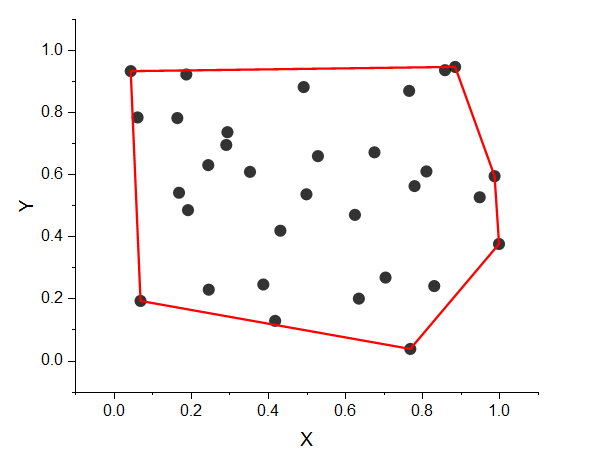
\includegraphics[width=\linewidth]{2D_ConvexHull}
	\end{column}
	\begin{column}{.6\linewidth}
	Q konvex burkát CH(Q)-val jelöljük.\\
$CH(Q)$-ra természetesen igaz, hogy $CH(Q) \subseteq Q$.
	\end{column}
\end{columns}
\end{frame}

\begin{frame}[fragile]{Konvex burok -- Graham-féle pásztázás}
\begin{alltt}
{\scshape{Graham-pásztázás}}(S) \{
  P0 = minimális y-koordinátájú Q-beli pont
  P=[P1 , P2, \ldots, Pm] Q pontjainak P0 körüli polárszöges rendezése
  S={\scshape{VermetLétesít}}()
  Verembe(P0, S)
  Verembe(P1, S)
  Verembe(P2, S)
  for i=3 to m \{
    while {\scshape{Legfelső-alatti(S)}}, {\scshape{Legfelső(S)}} és Pi pontok
szöge nem fordul balra \{
      {\scshape{Veremből(S)}}
    \}
    Verembe(Pi, S)
  \}
  return S
\end{alltt}
\end{frame}

\begin{frame}{Legtávolabbi pontpár megtalálása}
\begin{itemize}
	\item $n$ elemű ponthalmazban találjuk meg azon $(p_i, p_j)$ pontpárt, 
	melyek a legtávolabb fekszenek egymástól
	\item Nyers erővel $\binom{n}{2}=O(n^2)$
\end{itemize}
\begin{alertblock}{Észrevétel}
A ponthalmaz legtávolabbi pontpárja a CH-on található csúcspárok valamelyike 
kell legyen
\end{alertblock}
\end{frame}

\begin{frame}{Legtávolabbi pontpár megtalálása}
\begin{itemize}
	\item $n$ elemű ponthalmazban találjuk meg azon $(p_i, p_j)$ pontpárt, 
	melyek a legtávolabb fekszenek egymástól
	\item Nyers erővel $\binom{n}{2}=O(n^2)$
\end{itemize}
\begin{alertblock}{Észrevétel}
	A ponthalmaz legtávolabbi pontpárja a CH-on található csúcspárok 
	valamelyike 
	kell legyen
\end{alertblock}
\end{frame}

\begin{frame}{Legközelebbi pontpár megtalálása}
\begin{itemize}
	\item Adott $n$ elemű $P$ ponthalmazra mi az a $(p_i, p_j) \in Q \times Q$ 
	pontpár, ami a legközelebb helyezkedik el egymáshoz?
	\item Nyers erővel $\binom{n}{2}=O(n^2)$
	\item Oszd meg és uralkodj eljárással $O(n\log(n))$ is megoldható
\end{itemize}
\end{frame}

\begin{frame}{Legközelebbi pontpár megtalálása -- oszd meg és uralkodj}
\begin{itemize}
	\item Ha legfeljebb 3 pont maradt, akkor használjuk a nyers erő módszerét
	\item Egyébként hajtsuk végre a következőket
	\begin{itemize}
		\item Vegyük azt az $l$ egyenest, ami két egyenlő részre vágja a 
		pontokat ($P_L$ és $P_R$)
		\item A $P_L$ és $P_R$-beli pontok közül rekurzívan keressük meg a 
		legközelebbi pontpárt $d=\min(d_L, d_R)$
		\item Döntsük el, hogy találni-e olyan $(p_i, p_j)$ pontpárt, melyre 
		$p_i \in P_L$ és $p_j \in P_R$, továbbá távolságuk $d' < d$
	\end{itemize}
\end{itemize}
\end{frame}

\begin{frame}{Legközelebbi pontpár megtalálása -- illusztráció}
\begin{columns}
	\begin{column}{.5\linewidth}
\begin{figure}
	\centering
	\includegraphics[width=\linewidth]{closepair}
\end{figure}
	\end{column}
	\begin{column}{.6\linewidth}
		\begin{block}<2>{Jó hír}
			%$S$ sávon belül sem kell minden pontpárt összehasonlítanunk \\
			Elegendő az $y$ koordináta alapján vett rendezés szerinti 7 
			rákövetkező ponttal összevetni az $S$-beli pontokat
		\end{block}
	\end{column}
\end{columns}
\end{frame}

\end{document}